\documentclass{article} % For LaTeX2e
\usepackage{nips14submit_e,times}
\usepackage{graphicx}
\usepackage{hyperref}
\usepackage{url}
%\documentstyle[nips14submit_09,times,art10]{article} % For LaTeX 2.09


\nipsfinalcopy
\title{Employing an HMM and Decision Tree to Predict Student Behavior}

\author{
Maximo Q.~Menchaca\\
Department of Atmospheric Science\\
518 ATG\\
\texttt{menchaca@uw.edu} \\
\And
John G.~Lee\\
Department of Physics \\
180 NPL Building \\
\texttt{jgl6@uw.edu} \\
}

% The \author macro works with any number of authors. There are two commands
% used to separate the names and addresses of multiple authors: \And and \AND.
%
% Using \And between authors leaves it to \LaTeX{} to determine where to break
% the lines. Using \AND forces a linebreak at that point. So, if \LaTeX{}
% puts 3 of 4 authors names on the first line, and the last on the second
% line, try using \AND instead of \And before the third author name.

\newcommand{\fix}{\marginpar{FIX}}
\newcommand{\new}{\marginpar{NEW}}

%\nipsfinalcopy % Uncomment for camera-ready version

\begin{document}


\maketitle

\begin{abstract}
An online tutoring system tracks student interactions as they learn. The tracked interactions can be used to predict future student performance. A decision tree and a Hidden Markov Model (HMM) were used in conjunction to determine the learning rate of a student. Output from the decision tree determined that the step duration provided valuable information gain on the training data. Within this paper, we develop a decision tree that splits on both the step duration and opportunity of the skill involved in the step to predict the probability a student achieves a first correct on a given problem. A Hidden Markov Model is used to predict the expected step duration at a given test data point, which is then plugged into the decision tree.
\end{abstract}

\section{Introduction}
This project was developed from the 2010 KDD Cup Challenge. The challenge is based off a database of student interactions with an online Cognitive Tutors system. The challenge specifically provides us with 5 high school level algebra datasets. These datasets are extremely large, with some containing thousands of students and 20 million total interactions. Within, each step the student encounters is logged. Associated with each step is the time spent, the problem unit, section, and name, the skill associated with this step, the number of times a student has encountered the relevant skill (called the "Opportunity"), and student queries. Either (1) the student does not know how to do the problem and asks for help (Hints), (2) the student inputs an incorrect answer (Incorrects), or (3) the student inputs a correct answer (Corrects). The goal of the challenge is to use the training portions of the dataset to predict whether or not a student will achieve a "Correct" on their first attempt at a step given in the test set, i.e., the first interaction of a student with a particular step is a "Correct" rather than a "Hint" or "Incorrect".

At face value, an intuitive structure to developing a successful algorithm is not difficult. As students progress through the dataset, one would expect the students to generally improve at their algebra skills throughout the year. If we expect students to do better later on in the year than earlier, the temporal nature of the data must be taken into account. Given the time series nature of the data, a Hidden Markov Model (hereafter HMM) seems a natural choice to generate predictions of student performance.

One could then develop an HMM that shows improving performance with time, and from this develop probabilities of getting a "First Correct". However, the dataset is not conducive to such a simple system.

\section{Proposed Methods}

\subsection{Hidden Markov Model}

A Hidden Markov Model is a time series where the states of the underlying system are unknown, or 'hidden'. For example, a dishonest casino could occasionally switch a fair die for a loaded die, and the goal of the unlucky gamblers is to determine when the casino has performed the switch. This involves determining (1) the probability a round of gambling has started with the fair or loaded die (the STARTING probability of each state), (2) the probability that the die are being switch (the TRANSITION probability of each state), and (3) the probability of each output from the die in each state (the EMISSION probability of each state). In the example above, a fair die would have an equal $\frac{1}{6}$ chance of emitting a 1,2,3,4,5,6, while the loaded die would have, say, a $\frac{1}{2}$ of rolling a 3.

In the problem we are considering for this paper, we hope to develop hidden states relating to the student's comprehension - our hidden states might be "Unknowledgeable", "Learning", and "Comprehension". From these hidden states, we emit the probability of getting a problem first correct - higher for higher states of comprehension. A possible blueprint is shown in Table \ref{HMMprop}.

\begin{table}[t]
\begin{center}
\begin{tabular}{ccc|c|ccc|cc}
\multicolumn{3}{c}{$\pi$} && \multicolumn{3}{c}{$T$} & \multicolumn{2}{c}{$E$}\\
UK & L & C & & UK & L & C & 0 & 1\\
& & & UK &0.8 & 0.2 & 0.00  & 0.6 & 0.4\\
1.0 & 0.0 & 0.0 & L & 0.02 & 0.85 & 0.13 & 0.45 & 0.55\\
&&& C & 0.01 & 0.01 & 0.98 & 0.15 & 0.85\\

\end{tabular}
\caption{A proposed Hidden Markov Model for a student's learning history.}\label{HMMprop}
\end{center}
\end{table}

In the template HMM shown, we expect to start in the "Unknowledgeable" state, which has a 40\% chance of getting a 0. However, the student progresses to the "Learning" state as they progress, which hives us a higher chance (55\%) of getting the problem first correct. Finally, the student progresses to the terminal "Comprehension" state. The transition and emission probabilities in the template could be modified upwards or downwards depending on the speed at which the student learns.

Rather than a hard coded HMM, we could use the Baum-Welch algorithm to develop transmission and emission matrices for each student and skill directly from the data.

\subsection{Limitations to the Naive Approach}

Of course, there are numerous obstacles to the methods described in this template. Ideally, one could adapt this rough blueprint to each student and skill, creating $T$ and $E$ matrices that allow us to predict student behavior. However, the data is sparse. Not all students see all skills. As a matter of fact, some students have as few as 12 data points total in the training datset. Even worse, students exist in the test set that are NOT in the training set. Similarly, there are skills that are present in the test subset that never appeared during training. Evidently, with new features in the test set, creating an HMM specific to each student and skill is a pipe dream.

A further limitation arises due to the binary nature of our predicted variable, "Correct First Attempt". Given two possible emissions, a naive model built to predict this variable could give us two possible hidden states (the third of Table \ref{HMMprop} would be superfluous) - "Correct" and "Incorrect". Where "Correct First Attempt" is 1, we must be in the "Correct" state, while if "Correct First Attempt" is 0, we must be in the "Incorrect" state. Such output is useless for application to our test data!

There are numerous other limitations inherent to our data set. The Markov Model assumption relies on data being sequential - something that is not necessarily true in our training data. Numerous gaps exist, and should be taken into account. And most frustratingly, much of the information associated with a step is not present in the test data at all - we are only given the "Opportunity", row in the full dataset, and problem name. We therefore must find a variable related to "Correct First Attempt" in order to provide more robust output from the Baum-Welch algorithm in developing our HMM.

\subsection{Decision Tree}









The duration of time a student spends on a particular problem and the number of times a student encounters a given skill seem to be good predictors of the ability of a student to answer correctly, as the former provides strong information gains, while the latter correlates well with student performance. Since we are not given the step duration in the test set, we use our HMM to predict this.

In conjunction, a decision tree is built from the training dataset using these two variables to predict “Correct First Attempt”. The generated probabilities from the HMM were used to predict likely states in the test set, and a decision tree was then used to predict the probability of a correct first attempt in the test set.


\section{Data preprocessing}
The data comes in the format of records from the tutoring program, 19 variables. These variables include Problem Section, Unit, Name, time spent on the problem, hint queries, and number of times a student encounters a particular skill. Student IDs and problem information were converted from strings to integers, while dates were converted to epoch time. Because multiple skills could be present for an individual problem, Knowledge Component (KC) skills were converted to a matrix with component values set to one if the skill is present in the problem and zero otherwise. Similarly the associated Opportunity variable was converted to a matrix but with component values set to the opportunity number if the skill is present in the problem and zero otherwise.

\section{Decision Tree}
\subsection{Implementation}
The goal of a decision tree is to partition the data into classes that give low entropy organization of the dependent variable. Some variables lend themselves better to splitting then others. For example, one would expect the variable 'Opportunity' to be a good variable to split on - the more times a student encounters a given variable, the better they should do. Another possibility is 'Step Duration' - the longer a student spends on a given step, the more trouble they may be having and the less likely it is they will do well. On the other hand, the variable 'Incorrects' would be an extremely poor variable to split on - if a student achieved ANY incorrects for a given step, obviously they must not have gotten their first attempt correct!

\subsection{Test, Results}
We implement a preliminary decision tree using the two variables 'Step Duration' and 'Opportunity'. The following two tables depict the two possible trees with this implementation. The parenthetical values is the count in each class - and Root = Opportunity/Root = Step Duration give the predicted y value.
\begin{table}[t]
\caption{Decision tree application to test data}
\begin{center}
\begin{tabular}{c|c|c|c|c|c|c|c}
\multicolumn{8}{c}{Root = Opportunity}\\
Duration & Empty & 1 $>$ 5 & 5 $>$ 15 & 15 $>$ 25 & 25 $>$ 50 & 50 $>$ 100 & 100 $>$ ...\\
& (202669) & (66137) & (113527) & (73460) & (109617) & (105889) & (138395)\\
\hline
empty (3268) & 0/1 (1912) & 0/0 (245) & 0/0(301) & 0/0 (139) & 0/0 (222) & 0/0 (265) & 0/0 (184)\\
1 $>$ 15 (471730) & 1/0 (118157) & 1/0  (28966) & 1/0 (61024) & 1/0 (41988) & 1/0 (64766) & 1/0 (65678) & 1/0 (91151)\\
15 $>$ 30 (148490) & 0/0 (36914) & 0/0  (13167) & 0/0 (21686) & 0/0 (13453) & 0/0 (20447) & 0/0 (19060) & 0/0 (23763)\\
30 $>$ 45 (65065) & 0/0 (17430) & 0/0  (6766) & 0/0 (9919) & 0/0 (5941) & 0/0 (8564) & 0/0 (7586) & 0/0 (8859)\\
45 $>$ 60 (35206) & 0/0 (9043) & 0/0 (4086) & 0/0 (5599) & 0/0 (3426) & 0/0 (4582) & 0/0 (4035) & 0/0 (4435)\\
60 $>$ ... (85935) & 0/0 (19213) & 0/0 (12907) & 0/0 (14998) & 0/0 (8513) & 0/0 (11036) & 0/0 (9265) & 0/0 (10003)\\
\end{tabular}
\end{center}
\end{table}

The raw entropy of the data is $H(Y)$= 0.78, and after applying our decision tree, we obtain similar values either way - $H(Y|\bf{Opp}|\bf{Duration}) \approx H(Y|\bf{Duration}|\bf{Opp})$ = 0.65. However, we can see that the predicted values are much different either way - there is just one positive prediction if we use a root of Step Duration - when the opportunity is empty! This indicates some lack of robustness in choosing bins for the opportunity, which can be confirmed by changing these bins (not shown). On the other hand, we see that a small step duration leads to positive prediction robustly across all opportunity classes.

Applying this binning to create predicted $y_{pred}$ = 'Correct First Attempt' leads to an RMSE of $||y - y_{pred}||_2$ = .284 for Root = Opportunity and = .45 for Root = Step Duration across the training set. We cannot apply the decision tree on its own to the test set, as the step duration is not given.

\section{Hidden Markov Model}
\subsection{Implementation}
A hidden Markov model (HMM) was implemented to track the learning curve of the individual students [1]-[2]. We assume our hidden state is whether the student is knowledgeable or not at the time i in order to predict the probability of getting the problem i+1 correct on the first attempt. The model requires the creation of a finite set of possible observations given the various preprocessed variables. 

\subsection{Test}
We have experimented with smoothing by applying the forward-backward algorithm to predict subsequent Correct First Attempt variables. Educated but rough assumptions were made about start, transition, and emission probabilities of the hidden and observed states. Observations at a given problem are split into three states based on (1) whether their first attempt on any problem was correct; (2) if not, whether they at least had more corrects than incorrects over their entire observation history, and (3) otherwise. The students are assumed to start in the unknowledgeable state with 99\% probability. The smoothed data then predicts a probability for observing the next Correct on First Attempt variable as a 1.

\subsection{Results}
The output probabilities are plagued by underflows, where the probability of being in a particular hidden model state after many steps is too small to be tracked. A simple fix is to try implementing using an arbitrary floating point python package like mpmath. Another possibility is trying to implement the forward/backward algorithm with log probabilities instead [2]. Currently, underflow errors are treated as non-predictive, a state that currently applies to approximately a third of students, but predictive states show a root-mean-square-error of .477. A few quick tests were performed stepping through different transition probabilites from the unknowledgeable state, see figure~\ref{fig:dunno}.

\begin{figure}[h]
\begin{center}
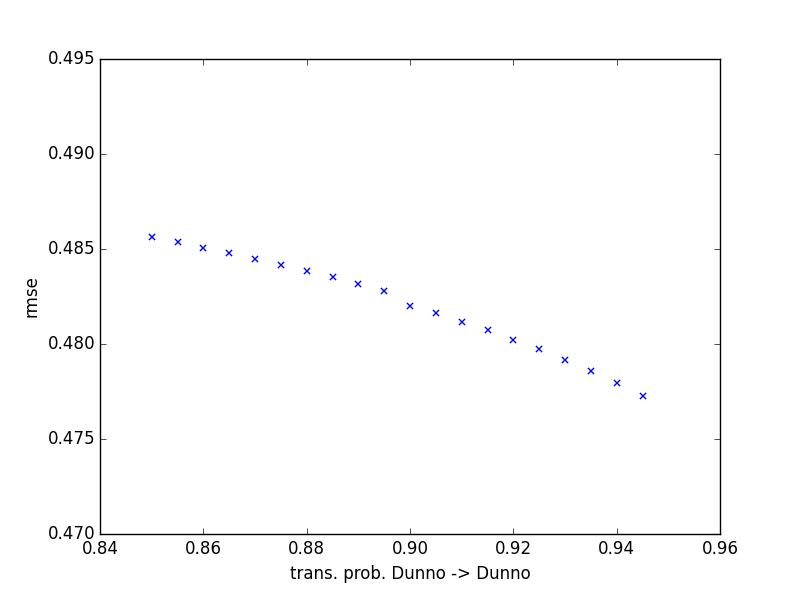
\includegraphics[width=0.8\textwidth]{dunno.png}
\label{fig:dunno}
\end{center}
\caption{Root-Mean-Square-Error with increasing probability of staying at unknowledgeable state from problem to problem.}
\end{figure}

\section{Conclusions}

The project gave us several insights into time allotment for a real-world type problem. Much of our time was spent trying to build these algorithms ourselves and test our functions which slowed down the process, but proved invaluable for comprehension of the methods and was somewhat fun. Additionally, a significant portion of the time was spent trying to understand the types of cases we could expect to see in the test data. We did not initially expect to find non-sequential questions in the test data relative to the training data, nor did we expect for their to be untracked students. So, a lot of time had to be allocated to parsing the data into a workable format, dealing with exceptions, and adjusting our plans for applying our HMM and decision tree. However, with all of that in mind, the vague strategy we started with was still able to be developed into a fitting plan.

The most important conclusion is that our goal in this situation where the test data does not exhibit all of the features of the training data is to generate reasonable features for the test data. In that way, an algorithm trained on the training data features can be applied to the test data. At the time of milestone our approach with the HMM was to generate an output at a subsequent time step of Correct First Attempt or not, which only yielded a guess slightly better than random. However, the best final results used the training data and HMM to predict a feature for the test data, Step Duration, that we knew to be fairly well correlated with the Correct First Attempt variable. We expect that generating more features in the test data would have yielded even better results. 

Additional ideas were proposed for extending the effectiveness of our methods. While our greatest succes came from predicting already tracked features of the data, e.g. step duration, we had also written a Viterbi algorithm which would have allowed us to track latent variables in the model between the training and test data. We also somewhat underutilized the ''Knowledge Component skills'' provided due to the sparsity of individual skills over multiple students. These ideas required more iterations of retraining and validating of the decision tree and HMM on components.


\subsubsection*{Acknowledgments}

Author MM acknowledges John G. Lee for his quality work thus far on the project described above. Author JL acknowledges Maximo Q. Menchaca for his quality work thus far on the project described above.

\subsubsection*{References}

\small{
[1] Frazzoli, E. (2010) Principles of Autonomy and Decision Making. 
\url{http://ocw.mit.edu/courses/aeronautics-and-astronautics/16-410-principles-of-autonomy-and-decision-making-fall-2010/lecture-notes/MIT16_410F10_lec21.pdf}\label{ref:hmmMIT}

[2] Domingos, P. (2015) \url{ http://courses.cs.washington.edu/courses/cse515/15wi/hmm.ppt}\label{ref:hmmUW}

[4] Lee, J.G.\& Menchaca, M.Q. (2015) Student Performance Prediction Using Hidden Markov Models and Decision Tree. CSE 546 Autumn 2015 Project Proposal, 1 pp., Unpublished.

[5] Guestrin, C. (2014) \url{ https://courses.cs.washington.edu/courses/cse546/14au/slides/decision-trees-annotated.pdf}

\end{document}